Distributed systems typically involve \emph{replication} of data
objects across a number of physical locations.  Replication is of
fundamental importance in such systems: it makes them more robust to
data loss and allows for good data locality.  But the well-known
\emph{CAP theorem}~\cite{gilbert-lynch-cap, BrewerCAPBlog} of
distributed computing imposes a trade-off between \emph{consistency},
in which every replica sees the same data, and \emph{availability}, in
which all
\ifdefined\DISSERTATION
\begin{wrapfigure}{r}{1.5in}
\vspace{-1em}
\begin{center}
  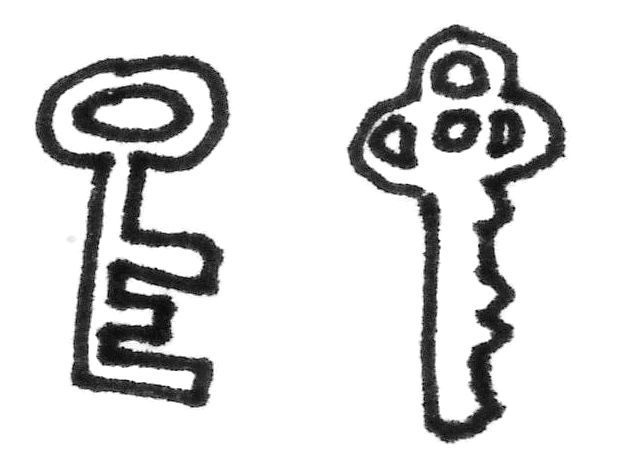
\includegraphics[scale=0.15]{../illustrations/keys}
\end{center}
\vspace{-1em}
\end{wrapfigure}
\fi
data is available for both reading and writing by all
replicas.  \emph{Highly available} distributed systems, such as
Amazon's Dynamo key-value store~\cite{dynamo}, relax strong
consistency in favor of \emph{eventual consistency}~\cite{vogels-ec},
in which replicas need not agree at all times.  Instead, updates
execute at a particular replica and are sent to other replicas
later. All updates eventually reach all replicas, albeit possibly in
different orders.  Informally speaking, eventual consistency says that
if updates stop arriving, all replicas will \emph{eventually} come to
agree.

Although giving up on strong consistency makes it possible for a
distributed system to offer high availability, even an eventually
consistent system must have some way of resolving conflicts between
replicas that differ.  One approach is to try to determine which
replica was written most recently, then declare that replica the
winner.  But, even in the presence of a way to reliably synchronize
clocks between replicas and hence reliably determine which replica was
written most recently, having the last write win might not make sense
from a \emph{semantic} point of view.  For instance, if a replicated
object represents a set, then, depending on the application, the
appropriate way to resolve a conflict between two replicas could be to
take the set union of the replicas' contents.  Such a conflict
resolution policy might be more appropriate than a ``last write wins''
policy for, say, a object representing the contents of customer
shopping carts for an online store~\cite{dynamo}.

Implementing application-specific conflict resolution policies in an
ad-hoc way for every application is tedious and
error-prone.\footnote{Indeed, as the developers of Dynamo have
  noted~\cite{dynamo}, Amazon's shopping cart presents an anomaly
  whereby removed items may re-appear in the cart!}  Fortunately, we
need not implement them in an ad-hoc way. Shapiro~\etal's
\emph{convergent replicated data types} (CvRDTs)~\cite{crdts,crdts-tr}
provide a simple mathematical framework for reasoning about and
enforcing the eventual consistency of replicated objects, based on
viewing replica states as elements of a lattice and replica conflict
resolution as the lattice's join operation.

Like LVars, CvRDTs are data structures whose states are elements of an
application-specific lattice, and whose contents can only grow with
respect to the given lattice.  Although LVars and CvRDTs were
developed independently, both models leverage the mathematical
properties of join-semilattices to ensure that a property of the model
holds---determinism in the case of LVars; eventual consistency in the
case of CvRDTs.  

CvRDTs offer a simple and theoretically-sound approach to eventual
consistency.  However, with CvRDTs (and unlike with LVars), it is
still possible to observe inconsistent \emph{intermediate} states of
replicated shared objects, and high availability requires that reads
return a value immediately, even if that value is stale.

In practice, applications call for both strong consistency and high
availability at different times~\cite{pileus}, and increasingly, they
support consistency choices at the granularity of individual queries,
not that of the entire system.  For example, the Amazon SimpleDB
database service gives customers the choice between eventually
consistent and strongly consistent read operations on a per-read
basis~\cite{simpledb-vogels-article}.

Ordinarily, strong consistency is a global property: all replicas
agree on the data.  When we make consistency choices at a
\emph{per-query} granularity, though, a global strong consistency
property need not hold.  I define a \emph{strongly consistent query}
to be one that, if it returns a result $x$ when executed at a replica
$i$:
\begin{itemize}
  \item will always return $x$ on subsequent executions at $i$, and
  \item will \emph{eventually} return $x$ when executed at \emph{any}
    replica, and will \emph{block} until it does so.
\end{itemize}
That is, a strongly consistent query of a distributed data structure,
if it returns, will return a result that is a \emph{deterministic}
function of all updates to the data structure in the entire
distributed execution, regardless of when the query executes or which
replica it occurs on.

Traditional CvRDTs only support eventually consistent queries.  We
could get strong consistency by waiting until all replicas agree
before allowing a query to return---but in practice, such agreement
may never happen.  In this chapter, I present an alternative approach
to supporting strongly consistent queries of CvRDTs that takes
advantage of their existing lattice structure and does \emph{not}
require waiting for all replicas to agree.  To do so, I take
inspiration from LVar-style threshold reads.  I show how to extend
CvRDTs to support deterministic, strongly consistent queries, which I
call \emph{threshold queries}.  After reviewing the fundamentals of
CvRDTs in Section~\ref{s:distributed-cvrdts}, I introduce CvRDTs
extended with threshold queries (Section~\ref{s:distributed-model})
and prove that threshold queries in our extended model are strongly
consistent queries (Section~\ref{s:distributed-results}).  That is, I
show that a threshold query that returns an answer when executed on a
replica will return the same answer every subsequent time that it is
executed on that replica, and that executing that threshold query on a
different replica will eventually return the same answer, and will
block until it does so.  It is therefore impossible to observe
different results from the same threshold query, whether at different
times on the same replica or whether on different replicas.
